\section{Эксперементальный раздел}

Для проведения тестирования был использован стандартный пакет Golang \textbf{testing}, также использовался подход
таблицоориентированного
тестирования, позволяющий обеспечить высокое покрытие кода, при меньших затратах на написание самих тестов.\cite{testdriven} 
\subsection{Тестирование компонент доступа к данным}

\begin{lstlisting}[caption=Тестирование компонент доступа к данным]
func TestProjectRepos(t *testing.T) {
    repos := []Repo{
        &TarantoolRepo{},
    }

    for _, repo := range repos {
        err := repo.Init("127.0.0.1", 6666)
        if err != nil {
            t.Errorf("Init on %T failed with %v", repo, err)
        }

        err = repo.Insert(&testProject)
        if err != nil {
            t.Errorf("Insert on %T failed with %v", repo, err)
        }

        err = repo.Insert(&testProject2)
        if err != nil {
            t.Errorf("Insert on %T failed with %v", repo, err)
        }

        proj, err := repo.GetByID(testProject.ID)
        if err != nil {
            t.Errorf("GetByID on %T failed with %v", repo, err)
        }
        if !testProject.IsEqual(proj) {
            t.Errorf("GetByID on %T expected %v, got %v", repo, testProject, proj)
        }

        proj, err = repo.GetByName(testProject.Name)
        if err != nil {
            t.Errorf("GetByName on %T failed with %v", repo, err)
        }
        if !testProject.IsEqual(proj) {
            t.Errorf("GetByName on %T, expected %v, got %v", repo, testProject, proj)
        }

        projs, err := repo.GetByOwnerID(testProject.OwnerID)
        if err != nil {
            t.Errorf("GetByOwnerID on %T failed with %v", repo, err)
        }
        if !testProject.IsEqual(&projs[0]) || !testProject2.IsEqual(&projs[1]) {
            t.Errorf("GetByOwnerID on %T, expected %v, got %v", repo, []models.Project{testProject, testProject2}, projs)
        }

        err = repo.DeleteByID(testProject.ID)
        if err != nil {
            t.Errorf("DeleteByID on %T failed with %v", repo, err)
        }

        err = repo.DeleteByName(testProject2.Name)
        if err != nil {
            t.Errorf("DeleteByName on %T failed with %v", repo, err)
        }
    }
}
\end{lstlisting}

\begin{lstlisting}[caption=Тестирование cлоя бизнес логики]
func TestProjectManagers(t *testing.T) {
    managers := []ProjectManager{
        &SimpleManager{},
    }

    ur := &user.TarantoolRepo{}
    sr := &schema.TarantoolRepo{}
    gr := &grant.TarantoolRepo{}
    pr := &project.TarantoolRepo{}
    tr := &task.TarantoolRepo{}
    ur.Init(host, port)
    sr.Init(host, port)
    gr.Init(host, port)
    pr.Init(host, port)
    tr.Init(host, port)
    for _, manager := range managers {
        err := manager.Init(ur, pr, gr, sr, tr)
        if err != nil {
            t.Errorf("Init failed on %T, with error %v", manager, err)
        }

        ur.Insert(&testOwnerUser)
        ok, err := manager.Create(&testProject)
        if err != nil {
            t.Errorf("Create on %T failed with error %v", manager, err)
        }
        if !ok {
            t.Errorf("Create on %T failed with not ok", manager)
        }

        ok, err = manager.Create(&testProject)
        if !ok {
            t.Errorf("Create after create on %T failed, with not ok", manager)
        }
        if err == nil {
            t.Errorf("Create after create on %T failed, with nil error", manager)
        }

        // AddUser to table
        ur.Insert(&testUser)
        ok, err = manager.AddGrant(testOwnerUser.Login, testProject.Project.Name, testUser.Login)
        if err != nil {
            t.Errorf("AddGrant on %T failed with error %v", manager, err)
        }
        if !ok {
            t.Errorf("AddGrant on %T failed with not ok result", manager)
        }

        ok, err = manager.DeleteGrant(testOwnerUser.Login, testProject.Project.Name, testUser.Login)
        if err != nil {
            t.Errorf("DeleteGrant on %T failed with error %v", manager, err)
        }
        if !ok {
            t.Errorf("DeleteGrant on %T failed with not ok result", manager)
        }

        ok, err = manager.AddGrant(testUser.Login, testProject.Project.Name, testOwnerUser.Login)
        if !ok {
            t.Errorf("AddGrant with wrong owner failed on %T, with no ok resp", manager)
        }
        if err == nil {
            t.Errorf("AddGrant with wrong owner failed on %T, expected not nil error", manager)
        }

        ok, err = manager.DeleteByName(testOwnerUser.Login, testProject.Project.Name)
        if err != nil {
            t.Errorf("DeleteByName failed on %T, with error %v", manager, err)
        }
        if !ok {
            t.Errorf("DeleteByName failed on %T, with not ok resp", manager)
        }

        err = ur.DeleteByLogin(testOwnerUser.Login)
        if err != nil {
            t.Errorf("Teardown failed on %T, error %v", manager, err)
        }
        err = ur.DeleteByLogin(testUser.Login)
        if err != nil {
            t.Errorf("Teardown failed on %T, error %v", manager, err)
        }
    }
}
\end{lstlisting}

\subsection{Тестирование GUI}

\begin{figure}[h!]
    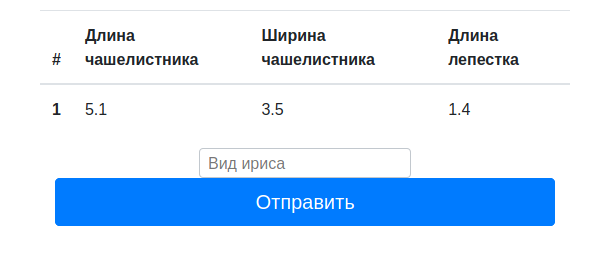
\includegraphics[width=0.9\textwidth]{./tablelabel.png}
    \caption{Экран разметки(таблица-текст)}
\end{figure}

\begin{figure}[h!]
    
\includegraphics[width=0.9\textwidth]{./animalslabel.png}
    \caption{Экран разметки(изображения-классы)}
\end{figure}

\begin{figure}[h!]
    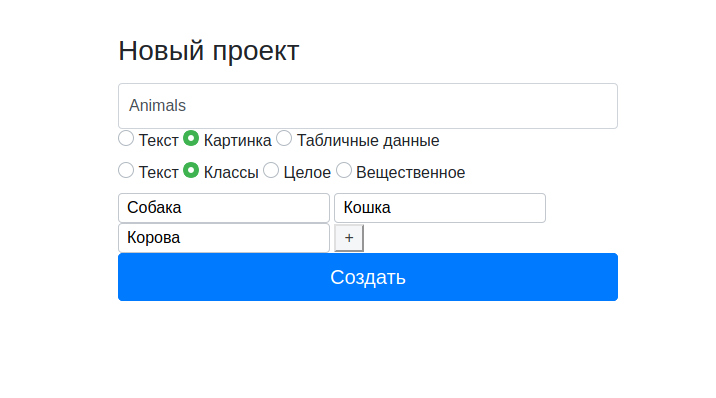
\includegraphics[width=0.9\textwidth]{./create_project.png}
    \caption{Экран создания проекта}
\end{figure}
